\appendixpage
\section{Sample Images Generated by Our Ray Tracing Program}

This section showcases sample images generated using our ray tracing program. These images demonstrate the program's capabilities and highlight the effects of varying parameters such as scene complexity, rendering resolution, and threading configurations.

\begin{figure}[htbp]
    \centering
    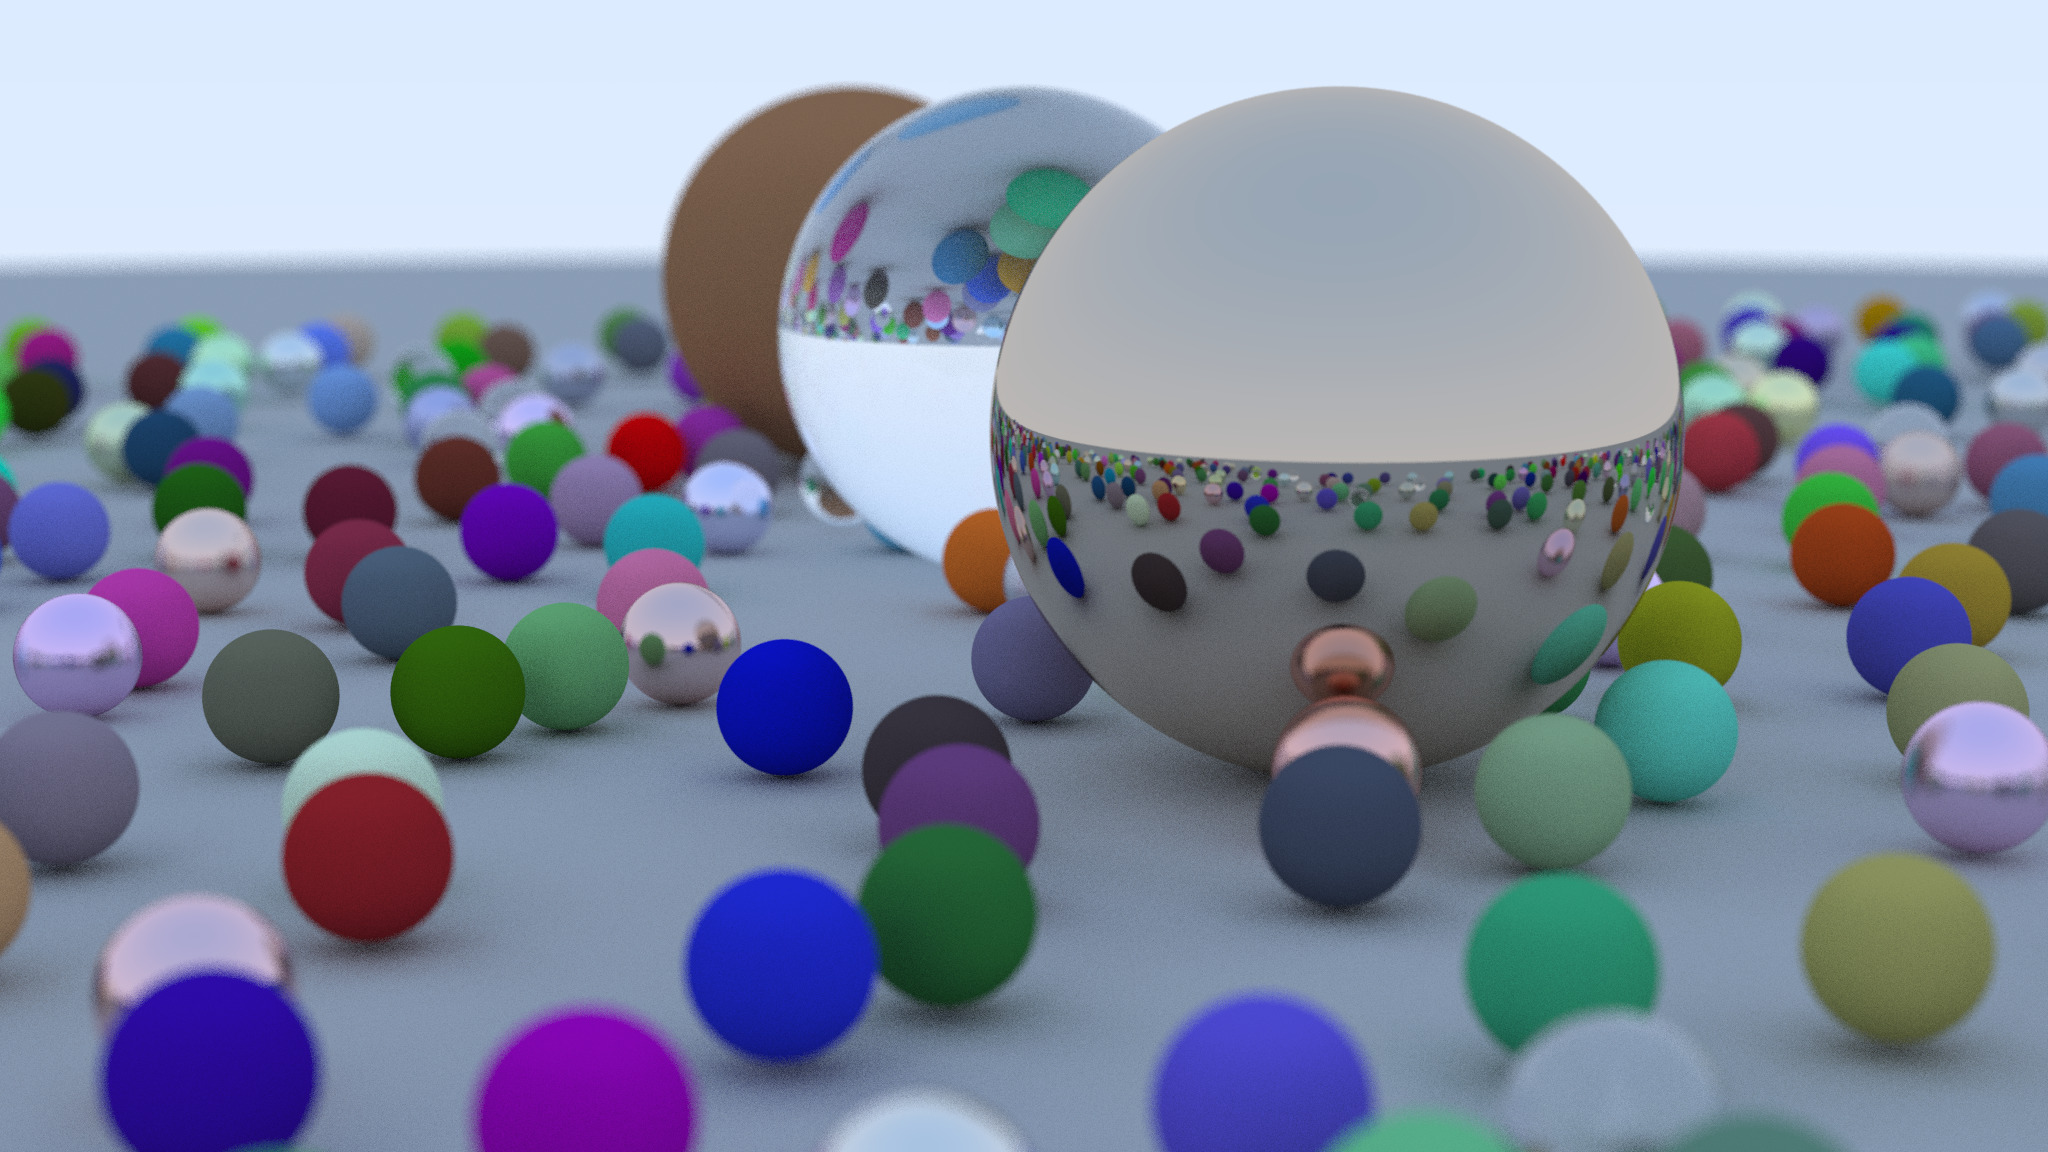
\includegraphics[width=1.0\linewidth]{images/fine-image.jpg}
    \caption{A high-quality image rendered with the following parameters: Samples per pixel = 32, Width = 2048, Height = 1152, Max Recursion Depth = 32, Scene Complexity = 11, Threads = 8, Schedule = Static. This example highlights the program's ability to handle complex scenes and produce detailed, photorealistic output.}
    \label{fig:sample-image-fine}
\end{figure}

The following figure compares scene complexity across three different configurations. Scene complexity determines the number of objects in the scene, which directly impacts rendering time and the level of detail in the output. A higher scene complexity results in more objects being rendered, creating a richer visual but also increasing computational demands.

\begin{figure}[htbp]
  \centering
  \begin{minipage}{0.3\textwidth}
    \centering
    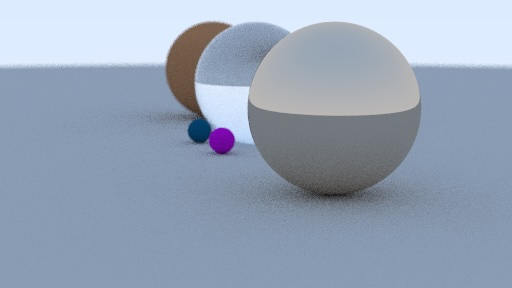
\includegraphics[width=\linewidth]{images/image-sphere-grid-1.jpeg}
    \subcaption{Scene Complexity = 1}
  \end{minipage}
  \begin{minipage}{0.3\textwidth}
    \centering
    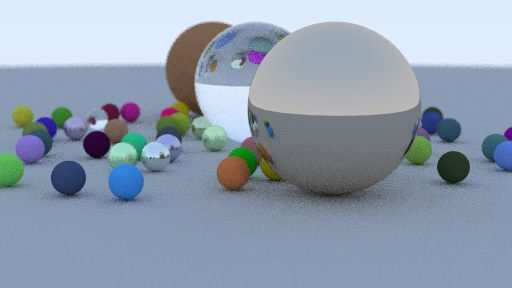
\includegraphics[width=\linewidth]{images/image-sphere-grid-4.jpeg}
    \subcaption{Scene Complexity = 4}
  \end{minipage}
  \begin{minipage}{0.3\textwidth}
    \centering
    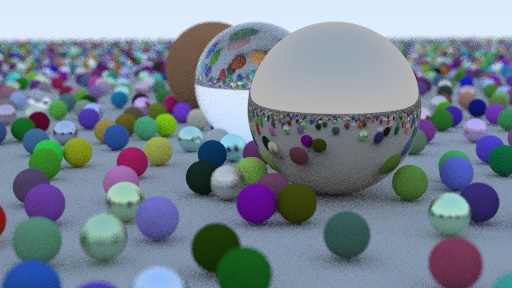
\includegraphics[width=\linewidth]{images/image-sphere-grid-64.jpeg}
    \subcaption{Scene Complexity = 64}
  \end{minipage}
  \caption{Illustration of scene complexity: (a) Scene Complexity = 1, (b) Scene Complexity = 4, (c) Scene Complexity = 64. As the complexity increases, the number of spheres in the grid grows, creating a more detailed and computationally intensive scene.}
  \label{fig:three_sphere_grids}
\end{figure}

\FloatBarrier
\section{Runtime Memory Footprint Investigation}
\label{sec:memory-footprint}

The memory footprint associated with different scene complexities, calculated at runtime, is shown in Table~\ref{tab:memory-footprint}. Each iteration (sampling a color for a ray) requires approximately 400 bytes per object for intersection testing in the current implementation. However, a detailed breakdown of the actual data needed for a single object reveals significant inefficiencies in memory usage. Optimizing the memory usage by minimizing overhead or restructuring data could dramatically reduce the memory footprint, leading to enhanced performance for large-scale scenes.

\begin{table}[htbp]
    \centering
    \small
    \begin{tabular}{|c|c|c|}
        \hline
        \textbf{Scene Complexity} & \textbf{Number of Small Spheres} & \textbf{Memory Footprint (KiB)} \\
        \hline
        1  & 4       & 1.5    \\
        16 & 1024    & 201    \\
        64 & 16384   & 3,276  \\
        \hline
    \end{tabular}
    \caption{Runtime Memory Footprint for the \texttt{world} at Different Scene Complexities.}
    \label{tab:memory-footprint}
\end{table}

\subsection{Minimum Memory Requirements for an Object}

The theoretical minimum size for a single object, based on the attributes used in intersection testing, is calculated as follows:
\begin{itemize}
    \item \textbf{Center coordinates:} 24 bytes (3 double-precision values)
    \item \textbf{Radius:} 8 bytes (1 double-precision value)
    \item \textbf{Material type:} 0.25 bytes (2-bit value, rounded for calculation)
    \item \textbf{Albedo:} 24 bytes (3 double-precision values)
    \item \textbf{Fuzz:} 8 bytes (1 double-precision value)
    \item \textbf{Refraction index:} 8 bytes (1 double-precision value)
    \item \textbf{Total Minimum Size:} 72.25 bytes
\end{itemize}

Considering hardware and compiler constraints, such as memory alignment or padding, this size may round up to the nearest memory block boundary, typically 8 or 16 bytes. This results in a practical memory usage of approximately 80 bytes per object.